% arara: lualatex
\documentclass{standalone}
\usepackage{mathtools}
\usepackage{unicode-math}
\unimathsetup{math-style=TeX}
\setmainfont{TeX Gyre Pagella}
\setmathfont{TeX Gyre Pagella Math}
% \documentclass[tikz]{standalone}
\usepackage{pgfplots}
\usetikzlibrary{arrows.meta}
\pgfplotsset{
    compat=1.10,
    width=9cm,
    height=7cm,
    % every tick/.style={color=black, semithick},
    % every minor tick/.style={thin},
    % axis line style = semithick,
    every axis/.append style={
        semithick,
        tick style = {color=black, semithick},
        minor tick style={thin},
    },
    legend style ={
        cells={anchor=west},
        draw=none,
        fill=none,
    }
}
\usepackage{mathtools}
\usepackage{unicode-math}
\unimathsetup{math-style=TeX}
\setmathfont[range=\mathup/{num}]{Times New Roman}
\setmathfont[range=\mathit/{greek,Greek,latin,Latin}]{Cambria Math}
\setmathfont[range=\mathup/{greek,Greek,latin,Latin}]{Cambria Math}
\setmainfont[Ligatures=TeX]{Times New Roman}
\setmonofont{Inconsolata}
\setmathfont[range={"2212,"002B,"003D,"0028,"0029,"005B,"005D,"221A,
"2211,"2248,"222B,"007C,"2026,"2202,"00D7,"0302,"2261,"0025,"22C5,
"00B1,"2194,"21D4,"2032}]
{Cambria Math}
\usepackage{siunitx}
\sisetup{%
    group-separator = {,} ,
    range-units = single ,
    range-phrase = {\text{--}} ,
    list-units = single ,
    list-separator = {\text{, }} ,
    list-final-separator = {\text{, and }} ,
    list-pair-separator = {\text{ and }} ,
    alsoload = synchem ,
    mode = text ,
}%
\DeclareSIUnit\calorie{cal}
\DeclareSIUnit\atmosphere{atm}

\usepackage[version=3]{mhchem}
\usepackage{chemfig}
\setatomsep{2.25em}
\usetikzlibrary{positioning, calc, arrows.meta}
\tikzset{
    flux/.style={right, align=left}
}
\newcommand*{\flux}[2]{\SI{#1}{\percent}\\\textit{\SI{#2}{\percent}}}
\usepackage{siunitx}
\sisetup{detect-all=true}

\begin{document}
    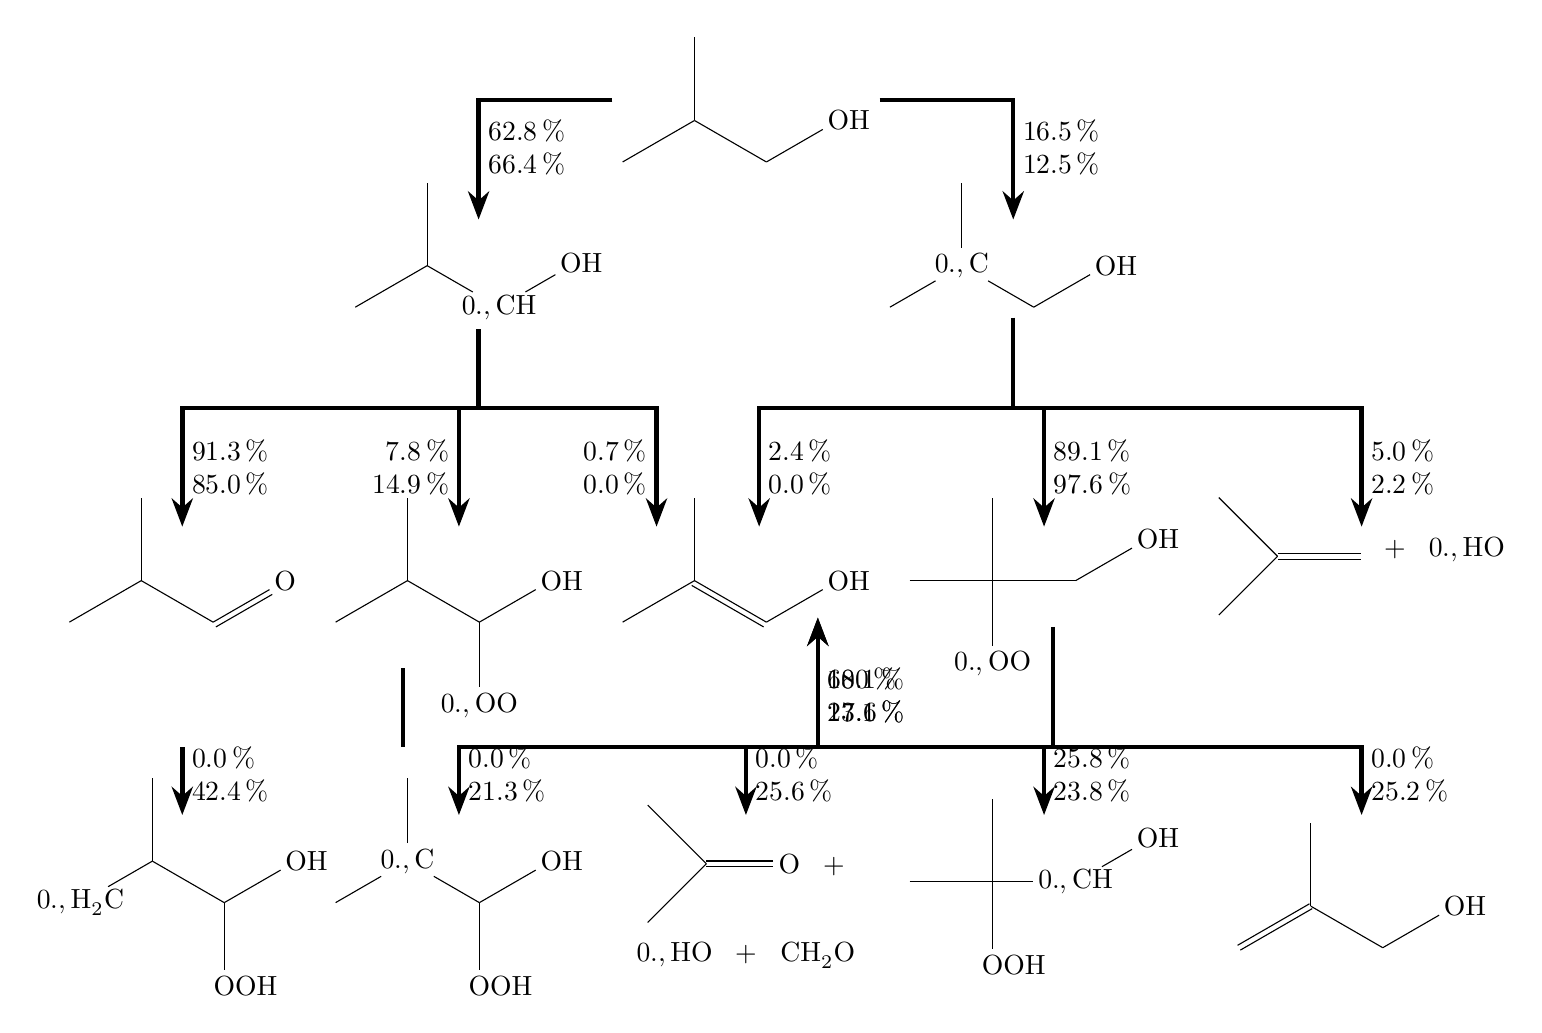
\begin{tikzpicture}[x=1cm, y=1cm, remember picture]
        \begin{scope}
            \node (ibuoh) {\chemfig{-[:30](-[2])-[:330]-[:30]OH}};
            \node[below left=0 and 0 of ibuoh] (aibuoh) {\chemfig{-[:30](-[2])-[:330]\lewis{0.,CH}-[:30]OH}};
            \node[below right=0 and 0 of ibuoh] (bibuoh) {\chemfig{-[:30]\lewis{0.,C}(-[2])-[:330]-[:30]OH}};
            \node[below=4 of ibuoh] (bibuohenol) {\chemfig{-[:30]@{enol-branch}(-[2])=_[:330]-[:30]OH}};
            \node[below=2 of bibuohenol, align=center] (scission) {\chemfig{[:180]O=(-[3])-[5]} \, $+$\\[0.5\baselineskip]\chemfig{\lewis{0.,HO}} \, $+$ \, \ce{CH2O}};
            \node[above left=0 and 0.25 of bibuohenol, anchor=north east] (aibuohoo) {\chemfig{-[:30](-[2])-[:330](-[6]\lewis{0.,OO})-[:30]OH}};
            \path let \p1 = (scission), \p2 = (aibuohoo) in node (aibuohbooh) at (\x2,\y1) {\chemfig{-[:30]\lewis{0.,C}(-[2])-[:330](-[6]OOH)-[:30]OH}};
            \node[above left=0 and 0.25 of aibuohoo, anchor=north east] (ibuohalde) {\chemfig{-[:30]@{alde-branch}(-[2])-[:330]=_[:30]O}};
            \path let \p1 = (scission), \p2 = (ibuohalde) in node (aibuohgooh) at (\x2,\y1) {\chemfig{\lewis{0.,H_2C}-[:30](-[2])-[:330](-[6]OOH)-[:30]OH}};
            \node[above right=0 and 0.25 of bibuohenol, anchor=north west] (bibuohoo) {\chemfig{-(-[2])(-[6]\lewis{0.,OO})--[:30]OH}};
            \path let \p1 = (scission), \p2 = (bibuohoo) in node (bibuohaooh) at (\x2,\y1) {\chemfig{-(-[2])(-[6]OOH)-\lewis{0.,CH}-[:30]OH}};
            \node[above right=0 and 0.25 of bibuohoo, anchor=north west] (isobutene) {\chemfig{[:180]=(-[5])-[3]} \, $+$ \, \chemfig{\lewis{0.,HO}}};
            \path let \p1 = (scission), \p2 = (isobutene) in node (gbutenol) at (\x2,\y1) {\chemfig{=[:30](-[2])-[:330]-[:30]OH}};
        \end{scope}

        \begin{scope}[every path/.style={draw, ultra thick, >={Stealth}}]
            \coordinate (first arrow end) at ($(aibuoh.north)-(0,0.6)$);
            \path[->] (ibuoh.west) -| (first arrow end) coordinate[pos=0.7] (first row);
            \path[->] let \p1 = (ibuoh.east), \p2 = (bibuoh), \p3 = (first arrow end) in (\x1,\y1) -| (\x2,\y3);

            \coordinate (second arrow end) at ($(ibuohalde.north)-(0,0.5)$);
            \coordinate (second row split) at ($(aibuoh.south)-(0,1)$);
            \path let \p1 = (aibuoh.south), \p2 = (second row split) in (\x1,\y1) -- (\x1,\y2);
            \path let \p1 = (bibuoh.south), \p2 = (second row split) in (\x1,\y1) -- (\x1,\y2);
            \path[<->] let \p1 = (second arrow end), \p2 = (second row split), \p3 = (bibuohenol.140), \p4 = (ibuohalde) in (\x4,\y1) -- (\x4,\y2) coordinate[midway] (second row) -- (\x3,\y2) -- (\x3,\y1);
            \path[<->] let \p1 = (second arrow end), \p2 = (second row split), \p3 = (bibuohenol.80), \p4 = (isobutene) in (\x4,\y1) -- (\x4,\y2) -- (\x3,\y2) -- (\x3,\y1);
            \path[->] let \p1 = (aibuohoo), \p2 = (second row split), \p3 = (second arrow end) in (\x1,\y2) -- (\x1,\y3);
            \path[->] let \p1 = (bibuohoo), \p2 = (second row split), \p3 = (second arrow end) in (\x1,\y2) -- (\x1,\y3);

            \coordinate (third arrow end up) at ($(ibuohalde.south)+(0,0.25)$);
            \coordinate (third arrow end dn) at ($(aibuohgooh.north)-(0,0.6)$);
            \coordinate (third row split) at ($(aibuohoo.south)-(0,0.25)$);
            \path let \p1 = ($(aibuohoo.245)+(0,0.75)$), \p2 = (third row split) in (\x1,\y1) -- (\x1,\y2);
            \path let \p1 = ($(bibuohoo.275)+(0,0.75)$), \p2 = (third row split) in (\x1,\y1) -- (\x1,\y2);
            \path[<->] let \p1 = (third arrow end dn), \p2 = (third row split), \p3 = (aibuohbooh), \p4 = (alde-branch), \p5 = (third arrow end up) in (\x4,\y5) -- (\x4,\y2) coordinate[pos=0.6] (third row up) -- (\x3,\y2) -- (\x3,\y1) coordinate[pos=0.4] (third row dn);
            \path[->] let \p1 = (third arrow end dn), \p2 = (aibuohgooh), \p3 = (third row split) in (\x2,\y3) -- (\x2,\y1);
            \path[<->] let \p1 = (enol-branch), \p2 = (third arrow end up), \p3 = (third row split), \p4 = (gbutenol.north), \p5 = (third arrow end dn) in (\x1,\y2) -- (\x1,\y3) -- (\x4,\y3) -- (\x4,\y5);
            \path[->] let \p1 = (scission), \p2 = (third arrow end dn), \p3 = (third row split) in (\x1,\y3) -- (\x1,\y2);
            \path[->] let \p1 = (bibuohaooh), \p2 = (third arrow end dn), \p3 = (third row split) in (\x1,\y3) -- (\x1,\y2);
        \end{scope}

        \path let \p1 = (first row), \p2 = (aibuoh) in node[flux] at (\x2,\y1) {\flux{62.8}{66.4}};
        \path let \p1 = (first row), \p2 = (bibuoh) in node[flux] at (\x2,\y1) {\flux{16.5}{12.5}};
        \path let \p1 = (second row), \p2 = (ibuohalde) in node[flux] at (\x2,\y1) {\flux{91.3}{85.0}};
        \path let \p1 = (second row), \p2 = (aibuohoo) in node[align=right, left] at (\x2,\y1) {\flux{7.8}{14.9}};
        \path let \p1 = (second row), \p2 = (bibuohenol.140) in node[flux, left] at (\x2,\y1) {\flux{0.7}{0.0}};
        \path let \p1 = (second row), \p2 = (bibuohenol.80) in node[flux] at (\x2,\y1) {\flux{2.4}{0.0}};
        \path let \p1 = (second row), \p2 = (bibuohoo) in node[flux] at (\x2,\y1) {\flux{89.1}{97.6}};
        \path let \p1 = (second row), \p2 = (isobutene) in node[flux] at (\x2,\y1) {\flux{5.0}{2.2}};
        \path let \p1 = (third row up), \p2 = (alde-branch) in node[flux] at (\x2,\y1) {\flux{100}{27.6}};
        \path let \p1 = (third row up), \p2 = (enol-branch) in node[flux] at (\x2,\y1) {\flux{68.1}{13.1}};
        \path let \p1 = (third row dn), \p2 = (aibuohgooh) in node[flux] at (\x2,\y1) {\flux{0.0}{42.4}};
        \path let \p1 = (third row dn), \p2 = (aibuohbooh) in node[flux] at (\x2,\y1) {\flux{0.0}{21.3}};
        \path let \p1 = (third row dn), \p2 = (scission) in node[flux] at (\x2,\y1) {\flux{0.0}{25.6}};
        \path let \p1 = (third row dn), \p2 = (bibuohaooh) in node[flux] at (\x2,\y1) {\flux{25.8}{23.8}};
        \path let \p1 = (third row dn), \p2 = (gbutenol) in node[flux] at (\x2,\y1) {\flux{0.0}{25.2}};
    \end{tikzpicture}
\end{document}
